% Unabridged Section 5.1 from Overleaf commit
% 1b194c68cc1b1cefc73c0126c192c0e59a464b5b.
% Archival LaTeX fragment: uses manuscript macros and cross-references.
% Not a standalone document.

\subsection{Infinitely many scales in one class}\label{sec:incommensurate-family}\label{sec:transcendental-dependence}
We allow different finite graphs in the three slots of the Wheatstone construction from Lemma~\ref{lem:permutation-obstruction}. Each resulting graph is then iterated as one fixed rule. The auxiliary tree below specifies the interior of that finite rule; it does not vary the rule between levels of the hierarchical lattice. The explicit graphs are large, so their allocations are supplied as finite integer certificates.

\begin{definition}\label{def:wheatstone}
The two-terminal Wheatstone skeleton has vertices $s,t,u,v$, terminals $s,t$, and edges $su,ut,sv,vt,uv$. Given terminal-symmetric two-terminal graphs $A,B,C$, let $W(A,B,C)$ replace $su,vt$ by fresh copies of $A$, $ut,sv$ by fresh copies of $B$, and $uv$ by a fresh copy of $C$. All interiors are disjoint. Write $E$ for a single edge and $W:=W(E,E,E)$.
\end{definition}

\begin{figure}[tbp]
\centering
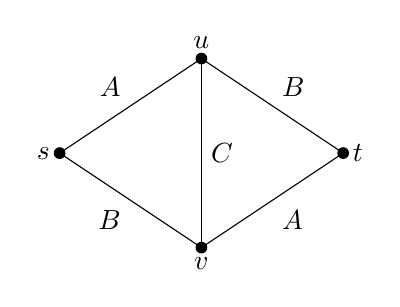
\begin{tikzpicture}[scale=1.2,vertex/.style={circle,fill=black,inner sep=1.5pt}]
\coordinate (s) at (0,0);\coordinate (t) at (3,0);
\coordinate (u) at (1.5,1);\coordinate (v) at (1.5,-1);
\draw (s)--node[above left]{$A$}(u)--node[above right]{$B$}(t);
\draw (s)--node[below left]{$B$}(v)--node[below right]{$A$}(t);
\draw (u)--node[right]{$C$}(v);
\foreach \p in {s,t,u,v}{\node[vertex] at (\p) {};}
\node[left] at (s){$s$};\node[right] at (t){$t$};
\node[above] at (u){$u$};\node[below] at (v){$v$};
\end{tikzpicture}
\caption{The Wheatstone substitution $W(A,B,C)$.}
\label{fig:wheatstone}
\end{figure}


All the graphs used here are built from $E$ by finitely many applications of $W$.

\begin{lemma}\label{lem:wheatstone-responses}
Every such graph other than $E$ is admissible and has critical point $1/2$. The operation satisfies
\begin{align*}
 m_{W(A,B,C)}&=2m_A+2m_B+m_C,\\
 \ell_{W(A,B,C)}&=\min\{\ell_A+\ell_B,2\ell_A+\ell_C,2\ell_B+\ell_C\},\\
 \varphi_{W(A,B,C)}'(1/2)
 &=\tfrac34\varphi_A'(1/2)+\tfrac34\varphi_B'(1/2)+\tfrac18\varphi_C'(1/2).
\end{align*}
Here $\varphi_E(p):=p$.
\end{lemma}
\begin{proof}
The simple terminal paths of the Wheatstone skeleton are $sut$, $svt$, $suvt$ and $svut$. Refining their edges proves the distance formula, and counting the five slots proves the edge formula. Every edge of a child graph lies on a simple terminal path of that child, and each skeleton edge lies on a simple terminal path of the skeleton. Concatenation proves canonicality. The two paths through $u$ and through $v$ give two edge-disjoint terminal connections, and every terminal path has at least two edges. No loops or parallel edges arise when fresh interiors are used. The involution $(s\ t)(u\ v)$ exchanges the paired copies of $A$ and of $B$ and reverses the copy of $C$; child terminal symmetry completes this involution.

At occupation $1/2$, induction makes the five child crossings independent fair bits. Exactly sixteen of the thirty-two skeleton configurations cross. Hence the parent crosses with probability $1/2$, which is its unique interior fixed point. Among the sixteen assignments of the other four bits, a fixed outer edge is pivotal in six and the central edge in two. Differentiating with respect to the five child crossing probabilities, then applying the chain rule, gives the thermal formula.
\end{proof}

The corresponding conditional mass kernels, obtained from the same thirty-two configurations, are
\begin{equation}\label{eq:wheatstone-kernels}
 \mathbf K_3:=\frac1{16}
 \begin{pmatrix}22&8&2\\10&14&8\\5&1&16\end{pmatrix},
 \qquad
 \mathbf J_3:=\frac1{16}
 \begin{pmatrix}9&5&2\\6&4&4\\3&1&4\end{pmatrix}.
\end{equation}
The first kernel counts a pair of opposite outer slots, and the second counts the central slot. Conditional independence inside the child graphs gives
\begin{equation}\label{eq:wheatstone-mass}
 \mathbf M_{W(A,B,C)}(1/2)
 =\mathbf K_3\mathbf M_A(1/2)
  +\mathbf K_3\mathbf M_B(1/2)
  +\mathbf J_3\mathbf M_C(1/2).
\end{equation}
Indeed, conditioning the skeleton fixes which child graphs cross, and therefore selects precisely the conditional child laws defining their matrix rows. The copies within a paired slot are already counted in $\mathbf K_3$. There is no additional factor of two in this formula.

\begin{definition}\label{def:leaf-allocation}
Start with a complete ordered ternary tree of depth $n$, interpreting its three branches as the slots $A,B,C$ of $W$. At each leaf place either $E$ or $W(E,E,E)$. Project a ternary leaf address to a binary word $\omega\in\{0,1\}^n$ by sending $A,B$ to $0$ and $C$ to $1$. If $z(\omega)$ is the number of zeroes, there are $2^{z(\omega)}$ ternary addresses with that projection.

An allocation consists of integers $x_\omega$ with $0\le x_\omega\le2^{z(\omega)}$. For each binary word, place $W(E,E,E)$ at the first $x_\omega$ of its ternary addresses in lexicographic order, with $A<B<C$, and place $E$ at the others. The resulting finite two-terminal graph is denoted by $R(n,x)$.
\end{definition}

An address describes a symbolic slot, while a slot of type $A$ or $B$ produces two physical copies. Keeping these two multiplicities separate is essential. A projected word with $z$ zeroes has $2^z$ available symbolic slots, each of which contributes $2^z$ physical leaf copies.

\begin{lemma}\label{lem:allocation-formulas}
For the graph $R(n,x)$,
\begin{align}
 \ell_{R(n,x)}&=2^n+x_{0^n},\label{eq:allocation-length}\\
 m_{R(n,x)}&=5^n+4\sum_{\omega}x_\omega2^{z(\omega)},\label{eq:allocation-volume}\\
 \varphi_{R(n,x)}'(1/2)
 &=\left(\frac{13}{8}\right)^n
   +\frac5{8^{n+1}}\sum_{\omega}x_\omega6^{z(\omega)}.\label{eq:allocation-thermal}
\end{align}
If $\mathbf P_\omega$ is the ordered product of $\mathbf K_3$ for each $0$ and $\mathbf J_3$ for each $1$, read from the root to the leaf, then
\begin{equation}\label{eq:allocation-mass}
 \mathbf M_{R(n,x)}(1/2)
 =(2\mathbf K_3+\mathbf J_3)^n+
 \sum_\omega x_\omega\mathbf P_\omega
 (2\mathbf K_3+\mathbf J_3-I).
\end{equation}
\end{lemma}
\begin{proof}
A subtree of height $r$ has terminal distance between $2^r$ and $2^{r+1}$. For three child subtrees of equal height, these bounds give $\ell_A+\ell_B\le2\ell_A+\ell_C$ and $\ell_A+\ell_B\le2\ell_B+\ell_C$. Thus the first branch of the minimum in Lemma~\ref{lem:wheatstone-responses} always attains the distance. The recursion follows only $A$ and $B$ slots, so each decorated leaf over $0^n$ adds one to the baseline distance $2^n$.

Replacing a leaf edge by $W(E,E,E)$ adds four edges and changes its thermal multiplier from $1$ to $13/8$. For a word with $z$ zeroes, the physical edge multiplicity is $2^z$, while the thermal weight along its symbolic address is $(6/8)^z(1/8)^{n-z}$. Summing these changes proves the volume and thermal formulas.

For a bare edge, $\mathbf M_E=I$. Repeated application of~\eqref{eq:wheatstone-mass} gives the baseline matrix $(2\mathbf K_3+\mathbf J_3)^n$. Changing one leaf replaces $I$ by $2\mathbf K_3+\mathbf J_3$ and left-multiplies this change by the ordered kernels along its address. Adding the changes proves~\eqref{eq:allocation-mass}. No permutation of the kernel factors is used.
\end{proof}

We first realise three rules with common critical dimensions and a common positive mass eigenvector. Their compositions will give an infinite family in the same class.
On the invariant plane $(a,2b,b)^T$, the integer numerators of the kernels in~\eqref{eq:wheatstone-kernels} act as
\[
 \mathbf K:=\begin{pmatrix}22&18\\5&18\end{pmatrix},\qquad
 \mathbf J:=\begin{pmatrix}9&12\\3&6\end{pmatrix},\qquad
 \mathbf D:=2\mathbf K+\mathbf J-16I
 =\begin{pmatrix}37&48\\13&26\end{pmatrix}.
\]
From this point onward, $\mathbf P_\omega$ denotes the ordered product of these integer matrices, so its denominator $16^n$ has been removed.
We seek allocations satisfying the four exact identities
\begin{align}
 x_{0^n}&=b^{100}-2^n,\label{eq:certificate-length}\\
 4\sum_\omega x_\omega2^{z(\omega)}&=b^{232}-5^n,\label{eq:certificate-volume}\\
 5\sum_\omega x_\omega6^{z(\omega)}&=8^{n+1}b^{70}-8\cdot13^n,\label{eq:certificate-thermal}\\
 \left[16(2\mathbf K+\mathbf J)^n+
 \sum_\omega x_\omega\mathbf P_\omega\mathbf D\right]
 \begin{pmatrix}55\\23\end{pmatrix}
 &=16^{n+1}b^{219}\begin{pmatrix}55\\23\end{pmatrix}.
 \label{eq:certificate-mass}
\end{align}
These are integer equalities, including the mass condition. The positive vector makes an eigenvalue check sufficient; a numerical estimate of the largest eigenvalue is unnecessary.

We specify the allocations compactly in two stages. The data are in the following directories, each containing \texttt{word\_base.json} and \texttt{packet\_repair.json}:
\begin{center}
\begin{tabular}{ccc}
\toprule
Base $b$ & Depth $n$ & Directory\\
\midrule
19 & 424 & \texttt{certificates/n424}\\
661 & 936 & \texttt{certificates/n936}\\
739 & 952 & \texttt{certificates/n952}\\
\bottomrule
\end{tabular}
\end{center}

The allocation files specify the initial counts as follows.
For each zero count $z$, \texttt{word\_base.json} gives two integer counts, indexed by the first letter of the word, and an integer lexicographic remainder. The initial value of $x_\omega$ is the count indexed by $z(\omega)$ and the first letter of $\omega$, plus one when $\omega$ precedes that remainder among all words with the same zero count. The file also records the sum of these values for each $z$.
There are $\binom{n-1}{z-1}$ words beginning with $0$ and $\binom{n-1}{z}$ beginning with $1$. These counts verify the recorded sums directly. Empty first-letter groups are omitted at $z=0,n$.

The second file prescribes corrections that leave distance, volume and pivotal response unchanged.
At each integer $t$ with $0\le t<n/4$, put $h:=2t+1$ and $L:=n-2h$. The file \texttt{packet\_repair.json} assigns one integer coefficient to each of the four tails
\[
 0^L,\qquad10^{L-1},\qquad1^L,\qquad01^{L-1}.
\]
Before each tail, place $h$ pairs, each independently chosen from $01$ and $10$. For every resulting word, add the assigned coefficient multiplied by $(-1)^{\text{number of }10\text{ pairs}}$ to its initial allocation.

Every such packet has a fixed zero count and total signed sum zero. It therefore preserves the volume and thermal sums, and it does not touch $0^n$, so it preserves the distance. Its ordered matrix contribution is explicit because
\[
 \mathbf K\mathbf J-\mathbf J\mathbf K
 =\begin{pmatrix}-6&-6\\3&6\end{pmatrix},\qquad
 (\mathbf K\mathbf J-\mathbf J\mathbf K)^2=18I.
\]
For its prescribed tail, the packet changes the mass numerator by its coefficient times
\[
 18^t(\mathbf K\mathbf J-\mathbf J\mathbf K)
 \mathbf P_{\mathrm{tail}}\mathbf D.
\]
This identity sums every word in the packet with its correct order and sign.

The packet supports are disjoint. At a fixed level their tails differ. Before the last level, $L\ge6$ and each tail has a pair $00$ or $11$ among its first two pairs. A higher-level packet would require both pairs to belong to $\{01,10\}$, so it cannot meet that support. Consequently capacity checks can be performed packet by packet. They use the distance of the two initial counts from $0$ and $2^z$, allowing for the possible remainder increment. When this uniform bound does not suffice, the finitely many affected words are checked individually.

\begin{lemma}\label{lem:integer-certificates}
The three allocations specified by these files satisfy
$0\le x_\omega\le2^{z(\omega)}$ for every word and satisfy
\eqref{eq:certificate-length}--\eqref{eq:certificate-mass} for
$(b,n)=(19,424),(661,936),(739,952)$.
\end{lemma}
\begin{proof}[Computer-assisted proof]
The verifier, \path{certificates/verify.py}, uses integer arithmetic throughout. It first enumerates the thirty-two skeleton configurations to reconstruct the original three-state kernels and the five pivotal counts. It then checks the initial group sizes, their totals and their capacities. The volume, thermal and distance assertions are the first three displayed integer identities.

For the mass identity, ordered products of the initial allocation are summed by a dynamic program indexed by word length and zero count. A lexicographic prefix is decomposed into complete word cylinders, so the remainder terms are also summed exactly. The program then adds the displayed matrix contribution of every correction packet. Capacity bounds suffice except for four words in the $19$ case, twelve in the $661$ case and twenty in the $739$ case; these words are explicitly enumerated. Disjointness of supports makes these checks cover the final allocation.

Finally the program lifts the result back to the original three-state vector $(55,46,23)^T$ and verifies~\eqref{eq:certificate-mass} by integer equality. The accompanying \texttt{verification.json} records successful checks and SHA-256 hashes of the input files. The verifier reads only the allocation data; it does not rely on numerical eigenvalues, floating-point tolerances, or the program that produced the data. This is a finite verification of the three specified instances, not a search used as evidence for a universal assertion.
\end{proof}

\begin{theorem}\label{thm:incommensurate-class}
There exist admissible rule graphs $R_{19},R_{661},R_{739}$ with critical point $1/2$ such that, for $b\in\{19,661,739\}$,
\[
 (\ell_{R_b},m_{R_b},\rho(\mathbf M_{\mathfrak C_{R_b}}),\varphi_{R_b}'(1/2))
 =(b^{100},b^{232},b^{219},b^{70}).
\]
Their critical mass matrices share the positive eigenvector $(55,46,23)^T$, and each generated lattice $\Xi$ satisfies
\[
 (\dim_{\mathrm H}(\Xi),\dim_{\mathrm M}(\mathfrak C),\dim_{\mathrm P}(\mathfrak C))
 =\left(\frac{58}{25},\frac{219}{100},\frac7{10}\right),
\]
while their scale logarithms are linearly independent over $\mathbb Q$.
\end{theorem}
\begin{proof}
Take the graphs $R(n,x)$ specified in Lemma~\ref{lem:integer-certificates}. Lemma~\ref{lem:wheatstone-responses} proves admissibility and the critical point. Substitution of the first three certificate identities into Lemma~\ref{lem:allocation-formulas} gives the stated distance, volume and thermal multiplier. The last certificate identity gives eigenvalue $b^{219}$ on $(55,46,23)^T$ for the original three-state matrix. Its positivity makes this eigenvalue the Perron root. The three logarithmic ratios give the displayed dimensions.

The integers $19,661,739$ are greater than one and pairwise coprime. An integer relation between their logarithms would give a product of integer powers equal to one. Taking a valuation at a prime dividing each base in turn forces each exponent to vanish. Multiplication of the logarithms by $100$ preserves this independence.
\end{proof}

These lattices belong to the same critical-exponent universality class by Theorem~\ref{thm:exponent-class-dimensions}, so their incommensurate scales disprove Conjecture~\ref{conj:scale-commensurability}.

\begin{example}
For $R_{19}$, direct substitution gives
\[
 \frac{\log(19^{232})}{\log(19^{100})}=\frac{58}{25},\qquad
 \frac{\log(19^{219})}{\log(19^{100})}=\frac{219}{100},\qquad
 \frac{\log(19^{70})}{\log(19^{100})}=\frac7{10}.
\]
Theorems~\ref{thm:critical-exponents-dimensions} and~\ref{thm:delta-eta-dimensions} give the four defining exponents
\[
 \beta=\frac{13}{70},\qquad
 \nu=\frac{10}{7},\qquad
 \delta=\frac{219}{13},\qquad
 \eta_{\mathrm{av}}=-\frac3{50}.
\]
The same calculation applies to $661$ and $739$. Despite this agreement, no positive numbers of substitution steps on any two of these lattices give equal length scales.
\end{example}

The common positive eigenvector makes the mass Perron roots multiplicative under these particular compositions. It is not a general property of substitution, as the noncommuting example in Section~\ref{sec:noncommuting} shows.
\begin{theorem}\label{cor:infinite-scales}\label{thm:infinite-incommensurate-scales}
For every integer $k\ge0$, there is a classical EIGS hierarchical lattice $\Xi$ with scale $(19\cdot661^k)^{100}$ and critical dimensions
\[
 (\dim_{\mathrm H}(\Xi),\dim_{\mathrm M}(\mathfrak C),\dim_{\mathrm P}(\mathfrak C))
 =\left(\frac{58}{25},\frac{219}{100},\frac7{10}\right).
\]
These scales are pairwise incommensurate.
\end{theorem}
\begin{proof}
Compose $R_{19}$ with $k$ copies of $R_{661}$ by uniform edge substitution. Composition preserves admissibility: terminal paths and the involution refine through the child graphs, and two edge-disjoint paths in each factor give two in the composite. All factors have critical point $1/2$, so the chain rule multiplies their thermal multipliers. Edge counts and distances multiply by the composition identities~\eqref{eq:substitution-responses}.

Their critical mass matrices have the common positive eigenvector $(55,46,23)^T$. Their product therefore has that eigenvector with eigenvalue $19^{219}661^{219k}$, which is its Perron root. Thus the composite has the same three logarithmic dimensions and scale $(19\cdot661^k)^{100}$.

If two such scales with indices $k,l$ had equal positive integer powers, their $19$-adic valuations would make the two powers equal. Their $661$-adic valuations would then give $k=l$. The scales also grow without bound.
\end{proof}


As a further application, a variant of the same construction gives three transcendental critical dimensions that remain rationally proportional.

\begin{theorem}\label{thm:transcendental-dependent-dimensions}
There is a classical EIGS hierarchical lattice $\Xi$ whose three critical dimensions are all transcendental but span a one-dimensional vector space over $\mathbb Q$. More precisely, its admissible rule $R$ with $p_c=1/2$ satisfies
\[
 (\ell_R,m_R,\rho(\mathbf M_{\mathfrak C_R}),\varphi_R'(1/2))
 =(19^{100}+480,19^{232},19^{219},19^{70}),
\]
and hence
\[
 (\dim_{\mathrm H}(\Xi),\dim_{\mathrm M}(\mathfrak C),\dim_{\mathrm P}(\mathfrak C))
 =\frac{\log19}{\log(19^{100}+480)}(232,219,70).
\]
\end{theorem}
\begin{proof}
Use the depth-$424$ allocation in \path{certificates/transcendental}. It has the same grammar and mass kernels as Definition~\ref{def:leaf-allocation}. The files specify a new initial allocation and new correction coefficients; changing the distance is not achieved by retaining the old allocation. The first certificate identity is now
\[
 x_{0^{424}}=19^{100}+480-2^{424},
\]
while the volume, pivotal and mass identities remain
\eqref{eq:certificate-volume}--\eqref{eq:certificate-mass} with $b=19$ and $n=424$.
The integer-only verifier \path{certificates/verify_transcendental.py} checks these identities, every allocation capacity, and the original three-state eigenvector $(55,46,23)^T$, using the same exhaustive skeleton enumeration and disjoint-packet identities as Lemma~\ref{lem:integer-certificates}. Thus this is another finite admissible rule with exactly the displayed multipliers.

Since $\gcd(19,19^{100}+480)=1$, a rational equality
$\log19/\log(19^{100}+480)=a/b$, with positive integers $a,b$, would imply $19^b=(19^{100}+480)^a$, which is impossible by prime factorisation. This logarithmic ratio is therefore irrational. If it were algebraic, the Gelfond--Schneider theorem would make
$(19^{100}+480)^{\log19/\log(19^{100}+480)}=19$
transcendental, a contradiction. The ratio is transcendental, as are its three nonzero rational multiples. Their rational span has dimension one.
\end{proof}

In this example,
\begin{gather*}
 \dim_{\mathrm M}(\mathfrak C)=\frac{219}{232}\dim_{\mathrm H}(\Xi),\qquad
 \dim_{\mathrm P}(\mathfrak C)=\frac{35}{116}\dim_{\mathrm H}(\Xi),\\
 \dim_{\mathbb Q}\operatorname{span}_{\mathbb Q}
 \{1,\dim_{\mathrm H}(\Xi),\dim_{\mathrm M}(\mathfrak C),\dim_{\mathrm P}(\mathfrak C)\}=2.
\end{gather*}
Thus even three transcendental dimensions need not satisfy the rank condition in Theorem~\ref{thm:dimension-rank}. This example does not provide two incommensurate scales in a nonrational class: whether nonrationality of the critical dimensions forces commensurability remains a separate question.

